\begin{figure}[ht!]
  \centering

  \begin{subfigure}[t]{0.48\textwidth}
    \centering
    \begin{tikzpicture}[thick, scale=0.9, baseline=(current bounding box.north)]
      % unify bbox across BOTH subfigures
      \path[use as bounding box] (0,0) rectangle (7,5);

      \foreach \x in {0,...,7} {
        \foreach \y in {2,...,4} {
          \node at (\x,\y) [circle, draw=lightgray, fill=lightgray, minimum width=2pt] {};
        }
      }

      \draw[line width=0.3mm] (0,2) -- (5,3) -- (7,4) -- (2,3) -- cycle;
      \draw[line width=0.4mm, lightgreen] (0,2) -- (7,4);
      \draw[line width=0.3mm, orange]     (2,3) -- (5,3);

      \foreach \x in {2,...,5} \node at (\x,3) [circle, fill=orange, minimum width=4pt] {};

      \node at (1.1,3) [black]{$(0,0)$};
      \node at (5.9,3) [black]{$(\ell,0)$};
      \node at (0.5,1.6) [black]{$(-n,-1)$};
      \node at (6.5,4.4) [black]{$(\ell+n,1)$};
    \end{tikzpicture}
    \caption{Lattice polygons with fixed lattice diameter \mbox{(orange)} and \mbox{unbounded} Euclidean diameter (green).}
    \label{fig:unbounded_ed}
  \end{subfigure}\hfill
  \begin{subfigure}[t]{0.48\textwidth}
    \centering
    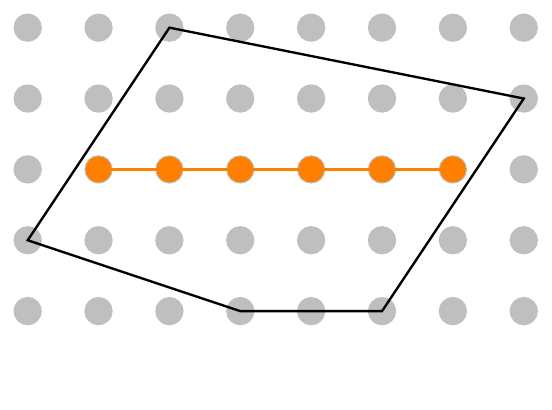
\begin{tikzpicture}[thick, scale=0.9, baseline=(current bounding box.north)]
      % unify bbox across BOTH subfigures
      \path[use as bounding box] (0,0) rectangle (7,5);

      \foreach \x in {0,...,7} {
        \foreach \y in {1,...,5} {
          \node at (\x,\y) [circle, draw=lightgray, fill=lightgray, minimum width=2pt] {};
        }
      }
      \draw[line width=0.3mm] (5,1) -- (7,4) -- (2,5) -- (0,2) -- (3,1) -- cycle;
      \draw[line width=0.3mm, orange] (1,3) -- (6,3);
      \foreach \x in {1,...,6} \node at (\x,3) [circle, fill=orange, minimum width=4pt] {};
    \end{tikzpicture}
    \caption{A lattice diameter segment contained in the interior of a lattice polygon.}
    \label{fig:LL_interior}
  \end{subfigure}

  \caption{Examples of lattice diameter segments in lattice polygons.}
  \label{fig:two_subfigs}
\end{figure}


% \begin{figure}[ht!]
%     \centering
%     % Left figure
%     \begin{minipage}[b]{0.48\textwidth}
%         \centering
%         \begin{tikzpicture}[thick, scale=0.9, baseline=(current bounding box.south)]
%             % unify bbox across BOTH figures
%             \path[use as bounding box] (-0.5,0.5) rectangle (7.5,5.5);

%             \foreach \x in {0,...,7} {
%                 \foreach \y in {2,...,4} {
%                     \node at (\x,\y) [circle, draw=lightgray, fill= lightgray, minimum width=2pt] {};   
%                 }
%             }

%             \draw[line width=0.3mm, black] (0,2) -- (5,3) -- (7,4) -- (2,3) -- cycle;
%             \draw[line width=0.4mm, lightgreen](0,2) -- (7,4);
%             \draw[line width=0.3mm, orange](2,3) -- (5,3);
            

%             \foreach \x in {2,...,5} {
%                 \node at (\x,3) [circle, fill=orange, minimum width=4pt] {};
%             }

%             % \node at (0,2) [circle, fill=black, minimum width=4pt] {};
%             % \node at (7,4) [circle, fill=black, minimum width=4pt] {};

%             \draw(1.1,3) node[black]{$(0,0)$};
%             \draw(5.9,3) node[black]{$(\ell,0)$};
%             \draw(0.5,1.6) node[black]{$(-n,-1)$};
%             \draw(6.5,4.4) node[black]{$(\ell+n,1)$};
%         \end{tikzpicture}
%         \caption{A lattice polygon with fixed \mbox{lattice} diameter (orange) and arbitrarily long \mbox{Euclidean} diameter (green).}
%         \label{fig:unbounded_ed}
%     \end{minipage}
%     \hfill
%     % Right figure
%     \begin{minipage}[b]{0.48\textwidth}
%         \centering
%         \begin{tikzpicture}[thick, scale=0.9, baseline=(current bounding box.south)]
%             % unify bbox across BOTH figures
%             \path[use as bounding box] (-0.5,0.5) rectangle (7.5,5.5);

%             \foreach \x in {0,...,7} {
%                 \foreach \y in {1,...,5} {
%                     \node at (\x,\y) [circle, draw=lightgray, fill= lightgray, minimum width=2pt] {};   
%                 }
%             }
%             \draw[line width=0.3mm, black] (5,1) -- (7,4) -- (2,5) -- (0,2) -- (3,1) -- cycle;

%             % segment
%             \draw[line width=0.3mm, orange](1,3) -- (6,3);

%             \foreach \x in {1,...,6} {
%                 \node at (\x,3) [circle, fill=orange, minimum width=4pt] {};
%             }
%         \end{tikzpicture}
%         \caption{A lattice diameter segment \mbox{in the interior} of a lattice polygon.}
%         \label{fig:LL_interior}
%     \end{minipage}
% \end{figure}
% % \begin{figure}[ht!]
% %     \centering
% %         \begin{tikzpicture}[thick, scale=1]\vspace{0.5cm}
% %         \draw[line width=0.3mm, white](-3,-1.5) -- (6,-1.5);
    
% %         \foreach \x in {-2,...,5} {
%             \foreach \y in {-1,...,1} {
%                 \node at (\x,\y) [circle, draw=lightgray, fill= lightgray, minimum width=1pt] {};   
%             }
%         }
    
%          \draw[line width=0.3mm, black] (-2,-1) -- (3,0) -- (5,1) -- (0,0)-- cycle;
%          \draw[line width=0.3mm, orange](0,0) -- (3,0);
%          \draw[line width=0.3mm, lightgreen](-1.9,-1) -- (4.9,1);

%          \foreach \x in {0,...,3} {
%                 \node at (\x,0) [circle, fill=orange, minimum width=4pt] {};
%             }
%         \node at (-2,-1) [circle, fill=black, minimum width=4pt] {};
%         \node at (5,1) [circle, fill=black, minimum width=4pt] {};

%         \draw(-0.8,0.3)node[black]{$(0,0)$};
%         \draw(4.1,-0.3)node[black]{$(\ell-1,0)$};
%         \draw(-1.6,-1.5)node[black]{$(-n,-1)$};
%         \draw(4.8,1.3)node[black]{$(\ell-1+n,1)$};
        

%     \end{tikzpicture} \vspace{-0.5cm}
    
%     \caption{unbounded Euclidean diameter for fixed lattice diameter}
%     \label{fig:unbounded_ed}
% \end{figure}